\documentclass[a4paper, titlepage]{article}
\usepackage[T1]{fontenc}
\usepackage[utf8]{inputenc}
\usepackage[english]{babel}
\usepackage{siunitx}
\usepackage{graphicx}
\usepackage{amsmath}
\usepackage{amsmath}
\usepackage{amssymb}
\usepackage{caption}
\usepackage{refstyle}
\usepackage{circuitikz}
\usepackage{subfig}
\usepackage{gensymb}
\usepackage{adjustbox}
\usepackage{latexsym}
\usepackage{float}
\usepackage{hyperref}
\usepackage[a4paper,top=2.5cm,bottom=2.5cm,left=2.5cm,right=2.5cm]{geometry}
%\usepackage[left=3cm, right=3cm, top=3cm]{geometry}

\usepackage{fancyhdr}
\pagestyle{fancy}
\lhead{}
\fancyhead[L]{\leftmark}
\lfoot{}
\cfoot{}
\rfoot{}
\rhead{\thepage}
%
\usepackage{rotating}
\usepackage{booktabs, longtable,afterpage}
\usepackage{rotating}
\usepackage{makecell}
\graphicspath{ {images/} }
\begin{document}
\begin{titlepage}
	\centering
	
\includegraphics[width=0.40\textwidth]{Politecnico_di_Torino_-_Logo}\par\vspace{1cm}
	\vspace{1cm}
	{\huge\bfseries Integrated Systems Architecture\par}
	\vspace{1cm}
	{\scshape\Large Lab 2: digital arithmetic \par}
	\vspace{2,5cm}
	{\Large\itshape Group 30:\\Chisciotti Laura 274728\\Fusto Federico 279925 \\Goti Gianluca 269825\par}
	\vspace{2,5cm}
		{\Large\bfseries Github repository: \url{https://github.com/Gotg3/ISA_Lab2.git}\par}
	\vfill

	\vfill
	{\Large A.Y. 20-21}
\end{titlepage}
\newpage
\tableofcontents
\newpage
\section{Introduction}
The goal of this lab is to deal with digital arithmetic issues.\\In particular it has been focused on a \textit{Floating point multiplier} with four pipeline stages. This multiplier has been handled in different ways. First of all, a layer of registers have been added at the input of the multiplier and then the Significands multiplier in Stage2 has been forced to be both a CSA multiplier and a PPARCH multiplier with the use of the Design Ware. For each case, a synthesis has been conducted to obtain the relative frequency and area.\\After that, the study has been focused on the fine-grain pipelining and optimization, where first, one register has been added at the output of the Significands multiplier in Stage2 and then more registers have been added up to six registers. Even for each of these cases, two syntheses have been done, one with the command \textbf{optimize\_registers} and the other one with the command \textbf{compile\_ultra} used for the optimizations.\\The last part of this lab is about the design of an \textit{MBE multiplier} that has been substituted to the behavioural operator '\textbf{*}' in the Significands multiplier in Stage2. For this case has been done every simulation and synthesis that have been carried out in the previous case, with the exception of the forcing to a CSA and PPARCH of the Significands multiplier in Stage2.
\section{Digital arithmetic and logic synthesis}
\subsection{Simulation}
Starting from a multiplier with four pipeline stages, a testbench has been created to perform some hexadecimal floating-point multiplications.
\\
%\\For both the multiplier's inputs have been given the same values which are hexadecimal samples contained inside the \textit{fp\_samples.hex} file.  (G)
Since the multiplier has been fed with the same inputs provided by the \textit{fp\_samples.hex} file, at the output the square values have been computed.
%these are available after 4 clock cycles compared to the corresponding input because the four pipeline stages have to be taken into account and this is possible to observe in Figure \ref{fig:sim_no_reg}.  L'ho spezzata mi sembra più pulita (G)
As one can see from Figure \ref{fig:sim_no_reg}, the results are available after 4 clock cycle with respect to the corresponding inputs since the pipeline stages have introduced an additional latency of 1 clock cycle each.
Then the obtained results have been compared with the values inside a supplied file: \textit{fp\_prod.hex}, which contains the square values of the inputs in hexadecimal format. The outputs of the simulation, which are reported in the first column of Table \ref{tab:output simulations}, have resulted as coincident with the values inside \textit{fp\_prod.hex} with the only difference that the undefined value "xxxxxxxx" has presented for five times before of the valid values and this has been caused because at the beginning the input is undefined for half clock cycle and this generates the first "xxxxxxxx" at the output, and then the four pipeline stages produce the other four undefined values before starting to give the correct values. 
\begin{figure} [h]
\centering
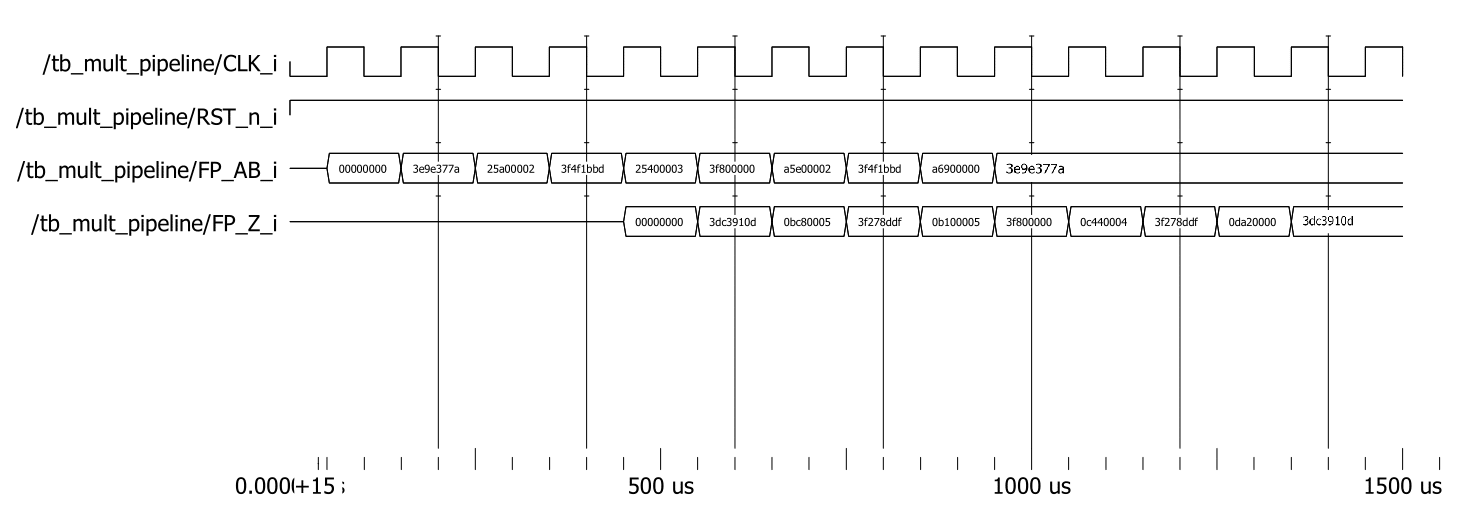
\includegraphics[scale=0.5]{print_sim_no_reg.png}
	\caption{Inputs and outputs of the pipeline multiplier}
	\label{fig:sim_no_reg}
\end{figure}
\noindent
\newline
After testing the right operation of the pipeline multiplier, a layer of registers have been added at the inputs of this one and another simulation has been carried out.\\The results of the simulation are reported in Figure \ref{fig:sim_inreg} and from this, it is possible to notice that the outputs have been shifted of a single clock cycle compared to the previous simulation in Figure \ref{fig:sim_no_reg}. This phenomenon has due to the presence of the registers which have been added at each input of the multiplier. In fact, in this case inside the output file with the hexadecimal output values, reported in the second column of Table \ref{tab:output simulations} , rather than having five values equal to "xxxxxxxx", six undefined values are present and then the correct square values are normally listed.
%there are not present five values equal to "xxxxxxxx" but six values of this one and then the right square values have been listed. (G)
\begin{figure} [h]
\centering
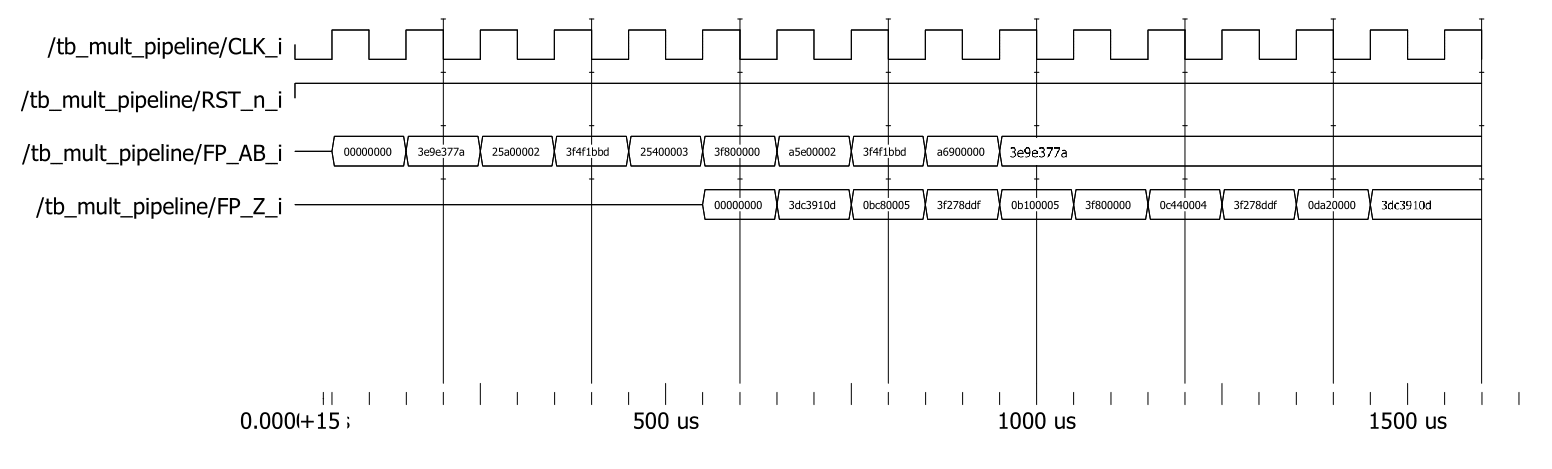
\includegraphics[scale=0.5]{print_sim_inreg.png}
	\caption{Inputs and outputs of the pipeline multiplier with an additional register}
	\label{fig:sim_inreg}
\end{figure}
\noindent
\subsection{Synthesys}
In this part, the Floating-point pipeline multiplier with an added register for each input has been synthesized in different ways.\\First of all this structure has been analyzed without changing anything and here this version is named as \textit{base version}. Therefore with Synopsys Design Compiler the hierarchy of the base version has been flattened and then this has been synthesized. From this procedure, the maximum frequency and the total cell area have been computed and these are equal to 632,9 MHz and 4057,8 $\mu m^2$ respectively, how it is possible to observe in Table \ref{tab:synthesys mult}.\\Afterward, the Significands multiplier in Stage2 has been handled to be a CSA and a PPARCH multiplier and to do that Design Ware (DW) has been exploited. % (G)
%has been used by Synopsys. Ho levato gli articoli ai nomi dei programmi con modelsim o quartus non abbiamo mai usato The
DW is a collection of ready-to-use blocks that contains even a parametric multiplier (DW02\_mult) that can be implemented as a \textbf{carry-save-adder} (CSA) or a \textbf{parallel-prefix architecture} (PPARCH).\\Thus Design Compiler first has been forced to use a CSA architecture for the Significand multiplier in Stage2 with the command \textbf{set implementation DW02 mult/csa [find cell *mult*]} after flattening the hierarchy. In this case, the maximum frequency and the total cell area have resulted as f$_{max}$=232,6 MHz and A$_{Tot Cell}$=4861,4 $\mu m^2$ as is reported in Table \ref{tab:synthesys mult}.\\In the end, the Stage2's Significand multiplier has been implemented as a PPARCH with the same procedure of the CSA but with using the \textbf{set implementation DW02 mult/pparch [find cell *mult*]} command and in this case f$_{max}$=606,1 MHz and A$_{Tot Cell}$=4009,4 $\mu m^2$ have been obtained and these results are even present in the last column of Table \ref{tab:synthesys mult}.
\\ For each case to compute the maximum frequency first it has been necessary to set the period equal to T=0 s, which gave a violated slack and then starting from this value a minimum period has been found to ensure a slack equal to zero. Therefore the inverse of the minimum period has been calculated to obtain the right value of each maximum frequency.\\At this point, observing all the values in Table \ref{tab:synthesys mult}, it is possible to compare the base version with the other two.\\Starting from the CSA case, where the module \textit{DW02\_mult} has been used, the maximum frequency is decremented compared with the f$_{max}$ of the base version, which is implemented as a PPARCH with using the module \textit{DW\_mult\_uns} of Design Ware, how is also reported inside the \textbf{resources report}. This decrease of the maximum frequency is caused by the fact that the insertion of the CSA in the path changes the delay which is become longer than before. Thus this generates a higher minimum period that goes from T$_{min}$=1,58 ns for the base version to T$_{min}$=4,3 ns for the CSA version which corresponds to a reduction in terms of frequency.
\\ Regarding the area, this is increased in the CSA case among the base version because one more block has been implemented to synthesize the CSA, in fact in the \textbf{report area} the value of the combinatorial part is increased from 2916,96 $\mu m^2$ (base version) to 3720,28 $\mu m^2$ (CSA version) and this could be even observed by the values of the Total cell area, reported in Table \ref{tab:synthesys mult}, that is higher for the CSA case compared to the base version.\\
The other case is the PPARCH and this has a maximum frequency as close as the maximum frequency of the base version and this is due to the fact that in both cases a parallel prefix approach is used with the only difference that in the base version the module \textit{DW\_mult\_uns} has been used as said before while in the PPARCH version has been implemented with the module \textit{DW02\_mult}.\\
Moreover, since for these cases the architecture is designed in a similar way, following the parallel prefix approach, even the value of the area is approximately the same, in fact, in the base version the Total cell area is equal to 4057,8 $\mu m^2$ while in the PPARCH version, it takes the value of 4009,4 $\mu m^2$ as reported in Table \ref{tab:synthesys mult}.

\section{Fine-grain Pipelining and optimization}
In this section, 
%it was asked to find the trade-off between the frequency achieved with the increase of the pipeline stages at the output of the Significands multiplier and the overall latency of the system.(L)
the trade-off between the frequency achieved with the increase of the pipeline stages at the output of the Significands multiplier and the overall latency of the system has been found. In order to do that two different commands 
%have been issued(non sono sicura che questo verbo sia giusto qui come significato) (L)
have been used, \textbf{optimize\_registers} and \textbf{compile\_ultra}. 
%Notice (L)
\\It is possible to notice that the Significands multiplier is still described as a generic multiplication "*", so the Synthesizer can choose automatically the best option for this component.
\newline
With the first command, 
%one can exploit the capability of optimizing of Design Compiler(L)
the capability of optimizing of Design Compiler can be exploited and after synthesized the circuit this command is able to optimize the architecture by means of \textbf{retiming}. Thus, it forces Design-Compiler to re-synthesize the design placing all the additional registers (at the output of Significands multiplier) in the proper locations to reduce the critical path.
\newline
The second command is a push-button solution for timing-critical and high-performance devices. It enables a routine that exploits several optimization tools such as automatic boundary optimization, automatic ungrouping, aggressive logic duplication for load isolation and many others.
\newline
Since the synthesis with these two additional commands required a discrete amount of time, only the base version of the 
%Multiplicands multiplier 
Significands multiplier has been studied. In this case, as it has been said, the multiplier has been described using a simple "*", leaving Design Ware free to choose the best option for it. In addition to the pipeline registers, at the output of the multiplier in Stage2, many other registers have been placed to ensure the correct behaviour of the stage. 
\newline
In this analysis up to six pipeline stages have been applied and the achieved results are reported in Figure \ref{fig:freq_comp}.


\begin{figure} [h]
\centering
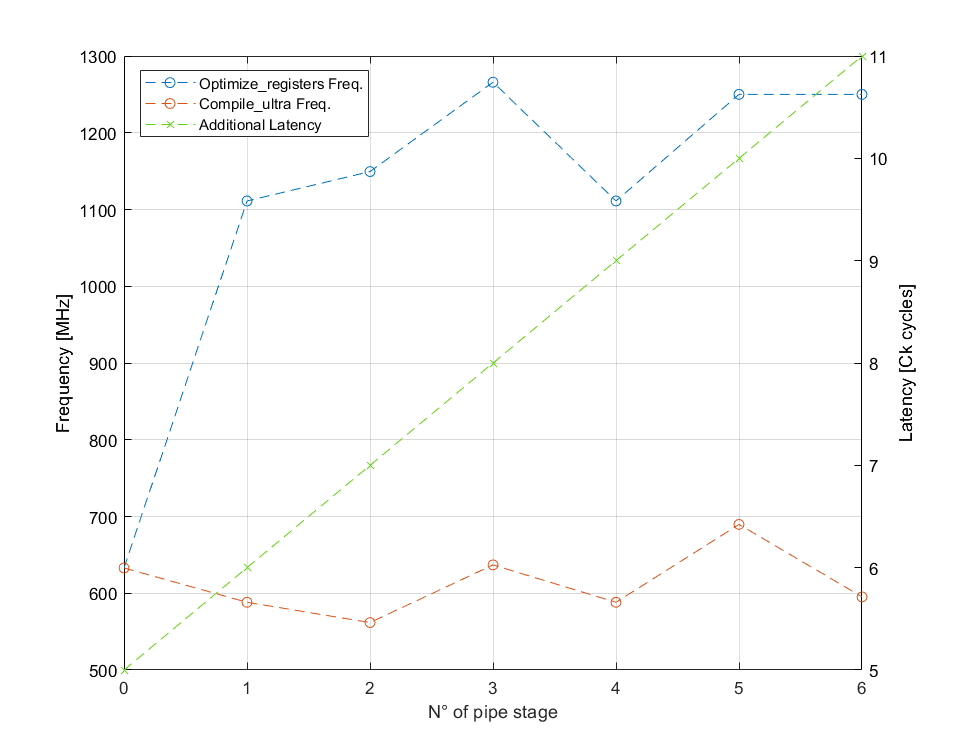
\includegraphics[scale=0.5]{freq_comp.png}
	\caption{Optimize\_registers freq. vs Compile\_ultra freq. }
	\label{fig:freq_comp}
\end{figure}

\newpage
\noindent
In this figure, for each number of pipeline stages is represented the corresponding frequency for both optimizations, the starting point "0" represents the base version of the multiplier with only the registers at the input of the architecture.
\newline
As one can see from this figure \textbf{optimize\_registers} command is much more effective than than \textbf{compile\_ultra}, with a frequency that on average is double starting from the first pipeline stage. From the graph it is clear that for an immediate improvement of the performance (and also a low additional latency) a good starting option is to use the \textbf{optimize\_registers} combined with a single pipeline stage at the output of the multiplier. In this analysis the maximum value is reached with 3 pipeline stages with a frequency equals to $f_{ck\; pipe 3}$=1265,82 MHz, obviously the latency has been increased of three clock cycle, so it is crucial to take into account this fact, according to the specific case where the architecture is involved. 
\newline
Starting from this point the frequency settles down, so any better improvement of the speed can be achieved using this type of command, with a higher number of pipeline stages.
\newline
On the contrary for the \textbf{compile\_ultra} command the frequency does not experience any great improvement, the maximum frequency is achieved with 5 pipeline stages and it is equal to  $f_{ck\; pipe 5}$=689,66 MHz. In this case the additional latency is not justified by the huge increasing of the frequency (like in the previous case) so it is preferable to not adopt this solution, probably all the applied methods are not so effective in this specific case with respect to retiming which has turned out to be very efficient even with a low degree of pipelining.
\newline
So in general it is important to find the best trade-off between clock frequency increasing and additional latency introduced in the design since, this latter increases linearly with the number of additional pipeline stages, as it is possible to observe in the plot.
\newline
In Table \ref{tab:freq_pipe_opt} all the frequency values for each number of pipeline stages have been reported, moreover it is possible to notice that it is also present the reference case with only the two input registers  (N° pipe= 0).
\newline
Concerning the area, all the values have been reported in Table \ref{tab:area_mult}, 
where there is even the percentage increase with respect to the 
reference design (with only the registers placed at the input).\\
As one can see from the table, the growth of the area is roughly double in the first optimization case (optimize\_registers). Thus, choosing this latter command, it is possible to increase the performance of the design with an increase of the area less than 50\%. While, if one of the constraints 
of the project is to save area, it is possible to adopt the second kind of optimization (compile\_ultra) that gives a low area increase but with also a low increase
of the operating frequency.
\\
Thus, depending on the adopted optimizing policy it is possible to focus the design on the performance or on the occupied area.
\newpage

\subsection{MBE Multiplier}
%aggiungo breve intro per passaggio da un argomento all'altro (L)
At this point of the lab, an unsigned MBE multiplier has been designed and used in Stage2 of the Floating point multiplier, instead of the behavioral description.\\ In particular the MBE multiplier consists of a Booth's encoding with a Radix-4 approach multiplier, that is the Modified Booth's encoding.\\
The needs to exploit both techniques comes to reduce the number of cycles required to compute the product from k to $\frac{k}{2}$ and the in-cycle-delay.\\
The Booth's encoding uses an extended digit set (0, 1, -1).\\Assuming that:
\begin{equation}
    P=A\cdot X 
\end{equation}
with $X=0001111_2=15_{10}$\\
\newline
Thus, the binary product consists of the following result:
\begin{equation}
    P=A\cdot(2^0 + 2^1 + 2^2 + 2^3)
\end{equation}
By translating the number into the new representation base method the X number is now X=001000-1.\\At this point the product P is computed as:
\begin{equation}
    P=A\cdot (2^4 - 2^0)
\end{equation}
This means that a reduction of number of operation needed is obtained by an increase of complexity to handle the new digit set.\\
The Radix-4 approach is basically used to reduce the length of the multiplicand A and the multiplier X so that the number of partial products could be halved.\\To do that, the new bit window used is $(x_{j+1}, x_{j})$, which assures an halving of iterations since now every partial product can express numbers from 0 to 4.
\\
Merging the two techniques together, the MBE is obtained.\\
The MBE is an extension of the Radix-2 approach. In fact in this case, instead of considering the multiplier on a bit-by-bit basis, more bits are analyzed simultaneously.\\Being the MBE a Radix-4 approach, it produces half partial products with respect to the Radix-2 solution and this leads to an improvement in %about (GG) 
the Dadda tree part because the height of each layer is reduced.
\newpage
\subsection{MBE multiplier's data path}
The architecture of the MBE multiplier is reported in Figure \ref{fig:datapath MBE}. From that, it is possible to observe that the MBE multiplier is implemented in a fully-parallel way. 
%in fact in the data path it is present the \textit{Dadda tree} structure that is typically used in the fully-parallel approach%

%Modifico perché frase abbastanza autoreferenziale e ridondante (FF) %

\begin{figure}[htp]
\centering
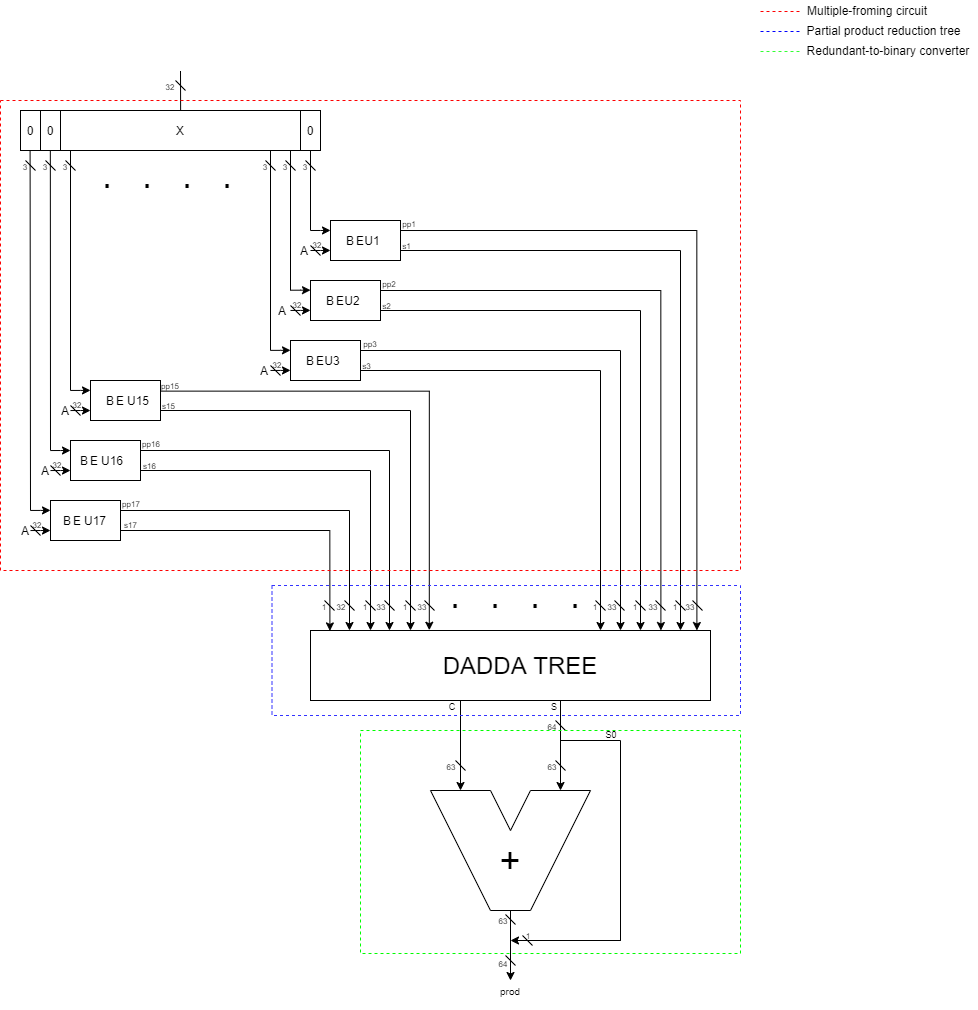
\includegraphics[scale=0.45]{Datapath_MBE_multiplier.png}
	\caption{MBE multiplier's data path }
	\label{fig:datapath MBE}
\end{figure}
\noindent
\newline
The architecture takes the multiplicand A and the multiplier X, both represented on 32 bits and it is composed of:
\begin{enumerate}
    \item The \textbf{X source}, to which 3 zeroes have been added, 1 on the right of the LSB
    %of X
    and the other 2 on the left of the MSB.\\
    %of X.\\
    %Forse si può levare "of X" dato che si parla di x così é meno ridondante
    These zeroes have been added to ensure %be sure to obtain 
    the correct number of triplets. Basing on every bits window values, the proper partial products have been selected using a multiplexer internally in the $B.E.U.$.
    %where each triplet corresponds to a partial product, 
    %therefore this procedure has been implemented to achieve the right number of partial products.%\\
    In the following figure (Figure \ref{tab:freq_pipe_opt}), it is possible to observe the internal layout of X after adding the zeroes and even how the triples have been taken. In particular, the total number of bits of this structure is partitioned in 3 bit windows with a 1-bit overlap.
    \newpage
    \begin{figure}[htp]
    \centering
    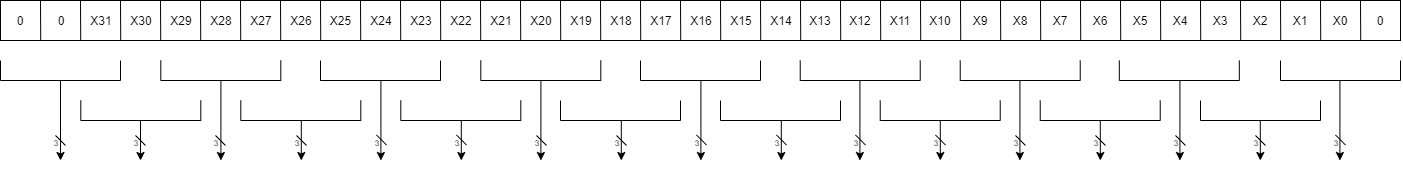
\includegraphics[scale=0.28]{x_triplets.png}
	\caption{Triplets' layout}
	\label{fig:X triplets}
    \end{figure}
   
	\item The \textbf{BEU block}, whose internal architecture is reported in Figure \ref{fig:BEU block}. This block is
	instantiated 
	17 times as the partial products required by the Dadda tree.\\
	The role of this block is to select the right value of the partial product (\textbf{pp}) between 0, A, 2A, -A, -2A and
	"-0" (implemented as \textbf{not(0)}) based on the bits window which are the bits that compose the selection signal. Moreover, another output is the sign (\textbf{s}) of the partial product that has been taken from the MSB of the triplet, indicated as X$_{j+1}$. In fact, if this value will be equal to zero, the partial product will be positive and the sign will assume the value zero, otherwise if X$_{j+1}$=1 the partial product will be negative since the sign will be equal to one, %ho aggiunto questa frase
	this information has been used to perform the Sign extension technique.\\Another characteristic is that the resize and shift operations have been applied on the input A of the BEU block in order to represent the value 2A or -2A without overflow. In fact the inputs and outputs of the multiplexer are represented on 33 bits.\\The only exception is for the \textbf{BEU17} block that maintains 32 bits since it has to represent only 0 and A as the last bits window can be either "000" or "001".
	\begin{figure}[htp]
    \centering
    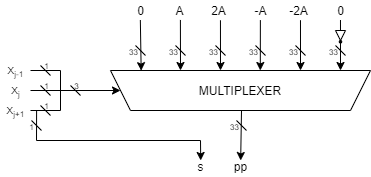
\includegraphics[scale=0.5]{BEU.png}
	\caption{BEU block}
	\label{fig:BEU block}
    \end{figure}
    \noindent
    \item The \textbf{DADDA TREE block}, which takes all the partial products and the signs and manage these to obtain carry on 63 bits and sum  on 64 bits at the output.
    \item The \textbf{Adder}, 
    it consist in a plain 63-bit adder which converts the redundant result into a normal binary representation.%that adds together all the carry bits with the sum bits from the 1 to 64.
    \\Then the result of the addition is concatenated with the LSB of the sum bits, S0, that is put as LSB of the final result, \textit{prod}.
\end{enumerate}
\subsubsection{Partial products generation}

The first layer in the MBE multiplier is the partial products generation path. 
\newline
It receives the multiplier X and extend it with a zero in the least significant position and two zeroes in the most significant positions. Then, each bits window $(x_{j+1}, x_{j}, x_{j-1})$ is selected from the output of the extended X and given as input to its relative $B.E.U.$,
which selects the correct operation.
The selection is based on a look-up table implementation.
\begin{center}
\begin{tabular}{c c c|c}
\multicolumn{1}{c}{$x_{j+1}$} &
\multicolumn{1}{c}{$x_j$} &
\multicolumn{1}{c|}{$x_{j-1}$} &
\multicolumn{1}{c}{operation}\\[0.8ex]
 \hline
0 & 0 & 0 & NOP \;(+0)\\
0 & 0 & 1 & +A\\
0 & 1 & 0 & +A\\
0 & 1 & 1 & +2A\\
1 & 0 & 0 & -2A\\
1 & 0 & 1 & -A\\
1 & 1 & 0 & -A\\
1 & 1 & 1 & NOP\;(-0)\\
\end{tabular}
\end{center}
\noindent
%The operation is then received by the MBE unit which outputs the partial product and its sign, used in the height reduction stages.
At this point, a partial product and its sign are issued from each BEU block.\\
The 
%MBE
BEU unit is the core of the implementation of this part, since it is instantiated as many times to cover the depth of 
%multiplier X. In the examined case X is represented on 32 bits, and having a windows sliding with 1 overlapping bit required 17 MBE units.
the extended multiplier X, that in the examined case comes from 32 bits of X to 35 bits of the extended version with the zeros inside. Thus, having a windows with 3 components sliding with 1 overlapping bit, 17 BEU units are required.\\
Finally, every partial product is paired with the corresponding root of the Dadda tree.

\subsubsection{Partial product reduction tree}

The adder plane relies on a Dadda-tree, which is a well-known structure for adding multiple operands. This is needed since in the fully-parallel tree approach, all the partial products are generated and provided to the adder simultaneously . 
\newline
In this structure the first task is to align data 
%ho aggiunto "in the first layer" (L)
in the first layer so that all the bits with the same weight are in the same column.
\\
%Layer after layer columns are compressed by means of "compressors" which are not other than Full-Adders (compress ratio 3/2) and Half-Adders (compress ratio 2/2), the overall structure is pictured (L)
Then, layer by layer, each column has been analysed and compressed if necessary by means of "compressors" which are not other than Full-Adders (compress ratio 3/2) and Half-Adders (compress ratio 2/2).\\Therefore, through this process, an overall structure has been obtained and this can be observed in Figure \ref{fig:dadda}.
\newline
Since the multiplier relies on the Radix-4 approach, the number of partial product is one half with respect to the basic Radix-2 approach and this is obtained by analysing more than one bit at the same time. 
\newline
In order to support the Booth's multiplication algorithm, it has been necessary to use the Sign Extension technique to compute all the needed sign extension constants.\\
Since some partial product can be negative, this approach allows managing % con allow manage prende -ing 
this situation by means of additional bits called S (sign bit) which can be either 1 or 0 depending on the value of the triplet which is being analyzed. In addition to that, an additional 1 is needed in the most significant position to convert back the string of ones to a leading of zeros. Then, the tree can be reduced in height and this operation gives the final result in Figure \ref{fig:dadda}. From this picture, it is possible to observe that, under the first 16 partial product, 
%is present the Sign bit related to the previous row, this bit is a 1 when the partial product is negative, this is necessary to convert the complemented partial product in the 2's complement version, while if the partial product is positive this bit is 0 son any modification is applied.
the Sign bit related to the previous row is present. In particular, this bit can be either a 1, when the partial product is negative and this is necessary to convert the complemented partial product in the 2's complement version, or a 0 if the partial product is positive, therefore any modification has to be applied.
\newline
In the specific case in which the triplet is equal to "111" the corresponding partial product would be "-0" and the sign would be 1 (negative p.p.). Since this latter is added to the previous partial product to obtain a row all equal to 0,
%is necessary to encode this specific partial product as a string of ones so that once they have been added the result is a string of zeros.
this specific partial product has to be encoded as a string of ones, thus that once that these are added together the result would be a string of zeros.
\newline
It is important to notice that all the partial products, except for the bottom one, have 33 bits since it is necessary to store also numbers as large as 2 times the multiplicand.
\newline
In the following, are reported all the levels with their correspondent height obtained according to the iterative rule of the Dadda-tree algorithm:
\begin{itemize}
    \item $l_0=2$
    \item $l_1=3$
    \item $l_2=4$
    \item $l_3=6$
    \item $l_4=9$
    \item $l_5=13$
    \item $l_6=17$
    
\end{itemize}
In each layer the Algorithm imposes to reduce the height by allocating the smallest number of HA's and FA's, it has turned out that in the structure are present:
\begin{itemize}
    \item HA: 45
    \item FA: 480
\end{itemize}
The final result of the Dadda-tree is in a carry-stored form since it has two outputs, the Carry vector (63 bits) and the Sum vector (64 bits).
\newline To obtain the usual binary result it is necessary to propagate these two vectors to a plain adder which converts the redundant representation into a binary one.
%\newline In this case, since in the least significant column only one dot was present, it has been taken as the true LSB of the final result while the remaining 63 bits have been propagated to the following building block which purpose is to compute the remaining part of the result.
    
    
    \newpage
    \begin{figure} [htp]
\centering
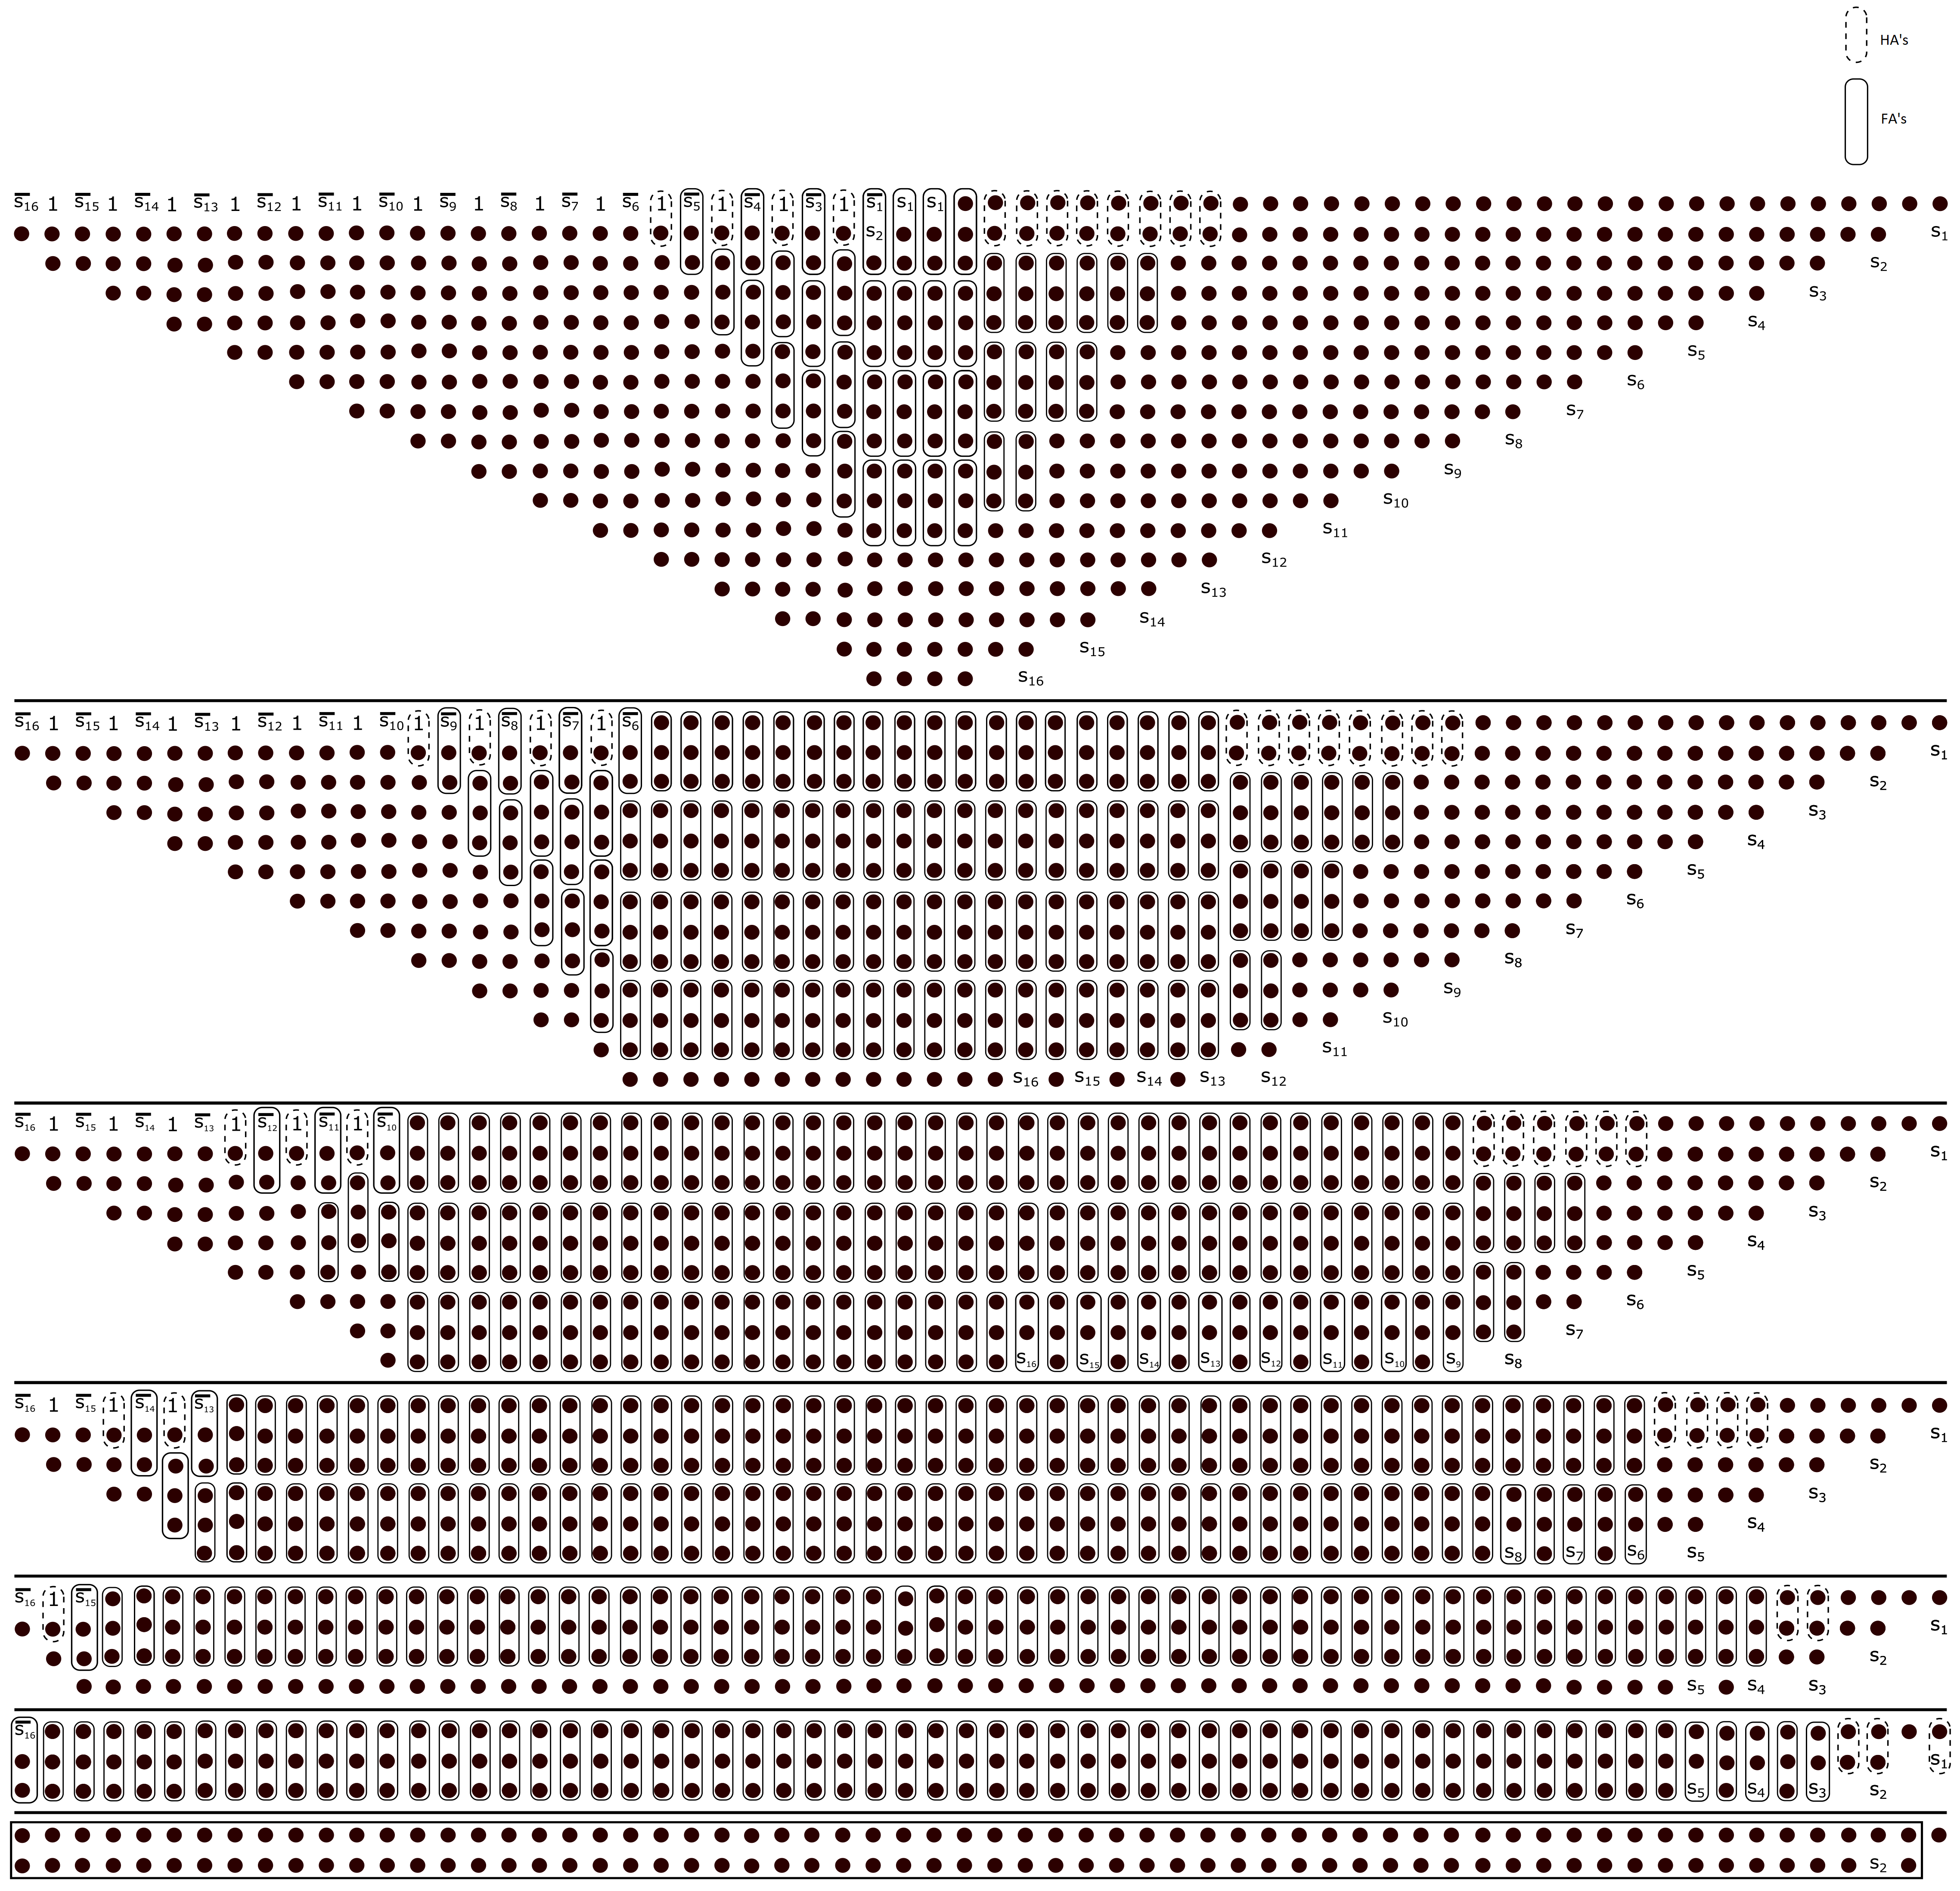
\includegraphics[scale=0.17]{dadda.png}
	\caption{Datta Tree Structure }
	\label{fig:dadda}
\end{figure}
    


\subsubsection{Redundant-to-binary converter}
The \textbf{redundant-to-binary convert} part, how it is possible to observe in Figure \ref{fig:datapath MBE} inside the green square, is made with an adder,
%aggiunto da qui
that is a converter form 2 operands to 1 operand.
%a qui
This in the VHDL code has been implemented in a behavioural way, simply writing the symbol '\textbf{+}' to add together the two inputs of the adder, which are all the 63 carry bits and the sum bits from the 1st to the 64th. This choice has been done in order to leave free Synopsys Design Compiler to implement the addiction with an adder block that it considers to be better than other possibilities.\\At the end of the computation, the result is concatenated with the LSB, S0, of the sum bits outgoing from the Dadda tree component, to generate the final output, \textit{prod}. Even for \textit{prod}, the bit S0 assumes the position of the LSB.
\newpage
\subsection{Simulation}
Once that the MBE multiplier has been implemented, this has been used to replace the behavioural operator '\textbf{*}' in the Significand multiplier in Stage2 of the Floating point multiplier. 
\newline
%After that the version of the Floating point multiplier with an added register at the input of this one and another register at the output of the Significand multiplier in Stage2 with respect to the initial version has been simulated to verify that the model was still working. 
After that the version of the Floating point multiplier with the additional registers at the input and the pipeline stage at the output of the Significand multiplier in Stage2 has been simulated to verify that the model was still working.
The results of the simulation are reported in Figure \ref{fig:sim_inreg_MBE}, from which it is possible to observe that the Floating point multiplier still works correctly because the output is present after six clock cycles with respect to the input and this is due to the fact that 4 pipeline stages, one register layer at the input and a pipeline stage at the output of the Significand multiplier in Stage2 are inserted along the path between the input and the output.
\begin{figure} [h]
\centering
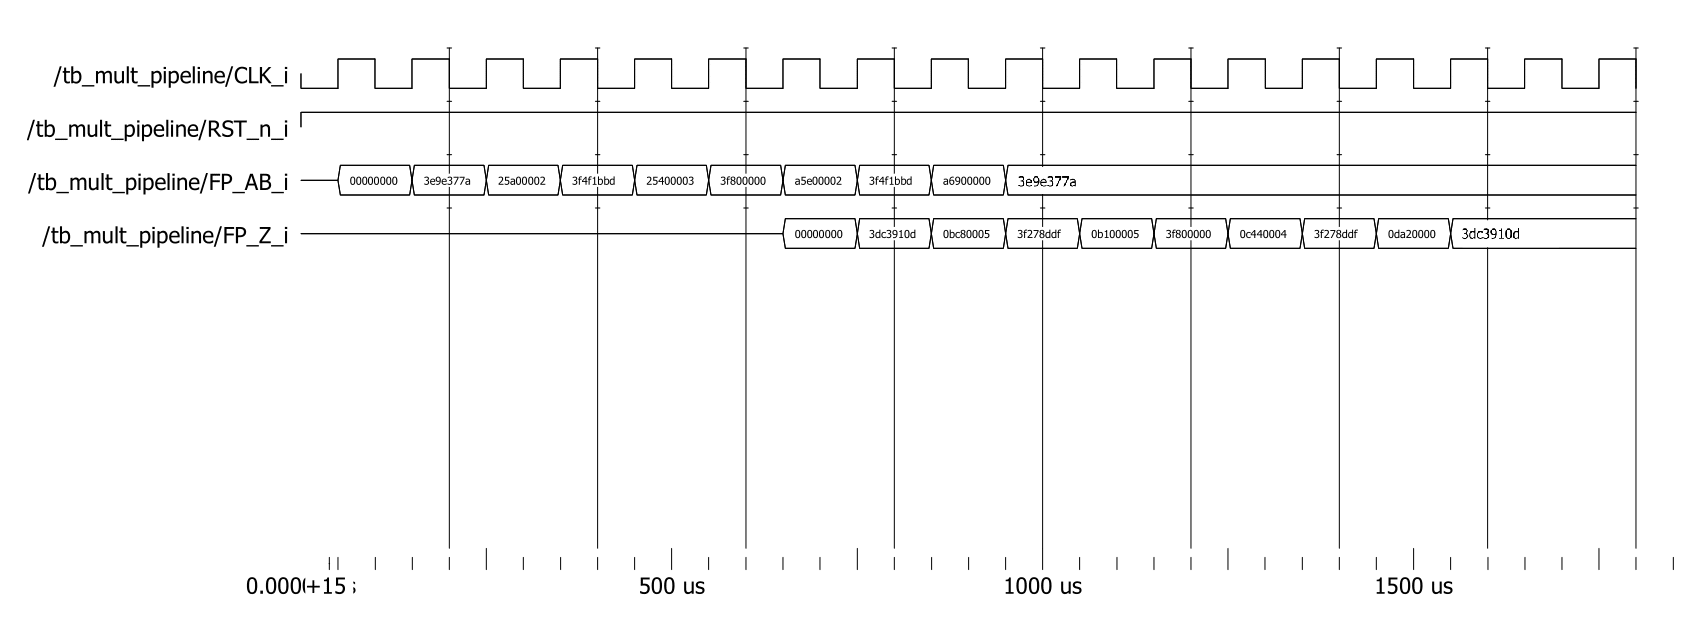
\includegraphics[scale=0.45]{print_sim_inreg_stage2_MBE.png}
	\caption{Inputs and outputs of the pipeline multiplier with MBE multiplier in Stage2}
	\label{fig:sim_inreg_MBE}
\end{figure}

\subsection{Synthesis}
As the previous case, in this section different types of optimization have been analyzed in order to find the best trade-off between frequency and latency. Also in this analysis, a maximum of 6 additional pipelining stages have been inserted.
\newline Notice that in this case, the analysis has been performed using from the beginning the registers at the input of the Floating point multiplier and an additional register at the output of the Significand multiplier in Stage2 (with all the other required registers to ensure the correct behaviour).
\newline
The new design has been synthesized using both compile optimization commands (\textbf{optimize\_registers} and \textbf{compile\_ultra}) starting from the beginning. \newline
Before proceeding into the full analysis, two different design solutions have been explored:
\begin{enumerate}
    \item Generic BEU block unit
    \item Custom BEU block unit
\end{enumerate}
This difference comes directly from the sign extension approaches where the last partial product is formed by 32 bits instead of 33 bits. Two different approaches have been exploited and analyzed, in the first one, one unique BEU block has been used and the last partial product (pp17) has been properly selected in order to have the correct parallelism (32 bits, discarding the MSB since this partial product can be either +0 or +A). In the second case, a custom BEU unit has been designed specifically for the partial product 17 where the only two possible selectable choices are +0 and +A (probably this solution is less demanding in terms of area). 
\newline
Therefore, these two different options have been synthesized and analyzed in order to find the best solution, 
%in Table \ref{tab:pp_17} are reported the different frequency values and in Table \ref{tab:area_pp_17} are reported all the Area values.
whose results are present in Table \ref{tab:pp_17} and in Table \ref{tab:area_pp_17}, where the different frequency values and the Area values have been respectively reported.\\
As one can see from the first Table, the multiplier with the generic BEU block ensures a faster implementation for both optimizations. Therefore, comparing the two implementations (custom and generic) in the \textbf{compile\_ultra} optimization, it is possible to observe that the generic case occupies a greater area, but this is reasonable because without a custom implementation the BEU unit is implementing a bigger multiplexer to handle the
six different inputs rather than only two.
%17 different inputs.
The design which has been adopted is the one with a generic implementation of the BEU block because it has led to a more effective increasing of the frequency. After the selection of the best design option, the analysis has proceeded through the study of the frequency improvement with respect to the additional pipeline stages insertion. 
In Figure \ref{fig:freq_MBE} is depicted the trend of the frequency with respect to the number of pipelining registers.


\begin{figure}[htp]
\centering
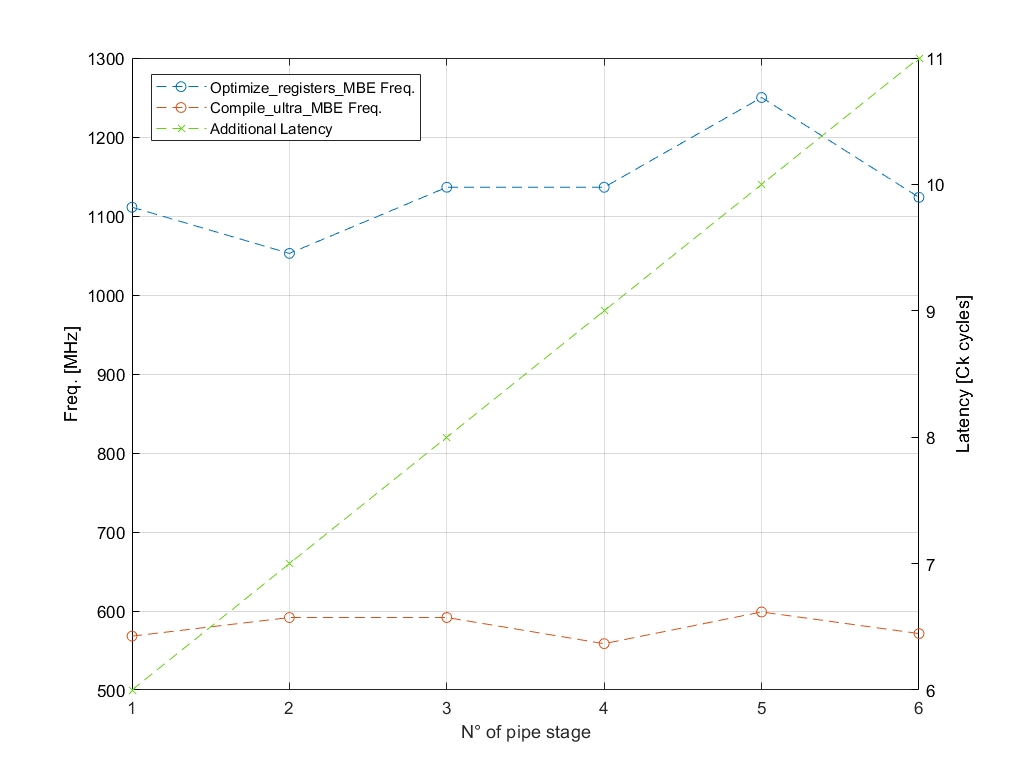
\includegraphics[scale=0.4]{freq_comp_MBE.png}
	\caption{MBE version: Optimize\_registers freq. vs Compile\_ultra freq.}
	\label{fig:freq_MBE}
\end{figure}
\noindent
%As one can see from the graph the command Optimize\_registers is capable to optimize in a more effective way the architecture in all the situations and the latency increases linearly with the number of the added pipelining stages.
\newline
\textbf{Compile\_ultra} command is not able to increase in an effective way the frequency of the multiplier, increasing the number of pipelining registers, actually, the frequency increasing is so limited that the addition of further pipeline stages leads to an unnecessary increase of latency.
\newline
On the contrary, \textbf{optimize\_registers} command is able to increase effectively the frequency, in fact it is roughly double than the previous optimization case starting from the beginning and the maximum is reached with 5 additional pipelining stages.
\newline
Data suggest that even with a single additional stage of registers it is possible to achieve a remarkable improvement of the frequency with the \textbf{optimize\_registers} command limiting at the same time the additional latency.
\newline
The latency (right axis of the plot) increases linearly with respect to the number of pipeline stages.
\newline
In Figure \ref{fig:MBE vs mult},
%are represented all the possible trends of frequency, 
all the possible trends of frequency are represented, comparing the base version with the generic multiplier and the "MBE" using both possible optimizations for each case.
\newline
Regarding the \textbf{compile\_ultra} case, the achieved frequency is in both version less than the other two versions where the optimization command has been applied.
The architecture which relies on the generic multiplier is capable to reach a slightly higher frequency compared with the one which uses the MBE multiplier. Anyway, both trend are very close and the maximum variation is $\simeq +15,2\%$ (base\_version frequency: 689,66 MHz vs MBE\_version frequency: 598,8 MHz)
achieved with 5 additional pipelining stages. 
\newline 
Comparing the generic multiplier result (N° pipe=5) with the reference value of 632,91 MHz (base\_version), which is obtained using a generic multiplier instead of its MBE version (N° pipe=0), it is possible to observe that the increase of frequency is only the $\simeq +8,9\%$. Thus, this has to be taken into account since to obtain such a small improvement it has been added a \textbf{not} negligible latency (+5 clock cycles of latency).
\newline

\noindent
With the \textbf{optimize\_registers} command the situation is completely different, starting from one additional pipelining case the achieved frequency is very high. The frequency trend of the  MBE version of the architecture is slower than the other one and it is able only in two cases to overcome or to match the original version.
In this latter specific case the two trends are equal only with 5 pipeline stages, therefore this is not a convenient choice since with 3 pipeline stages it is possible to obtain an higher frequency with a lower latency.
\newline Thus considering the frequency, the MBE version of the multiplier is not able to lead to any effective improvement of the performance of the system.

\begin{figure}[htp]
\centering
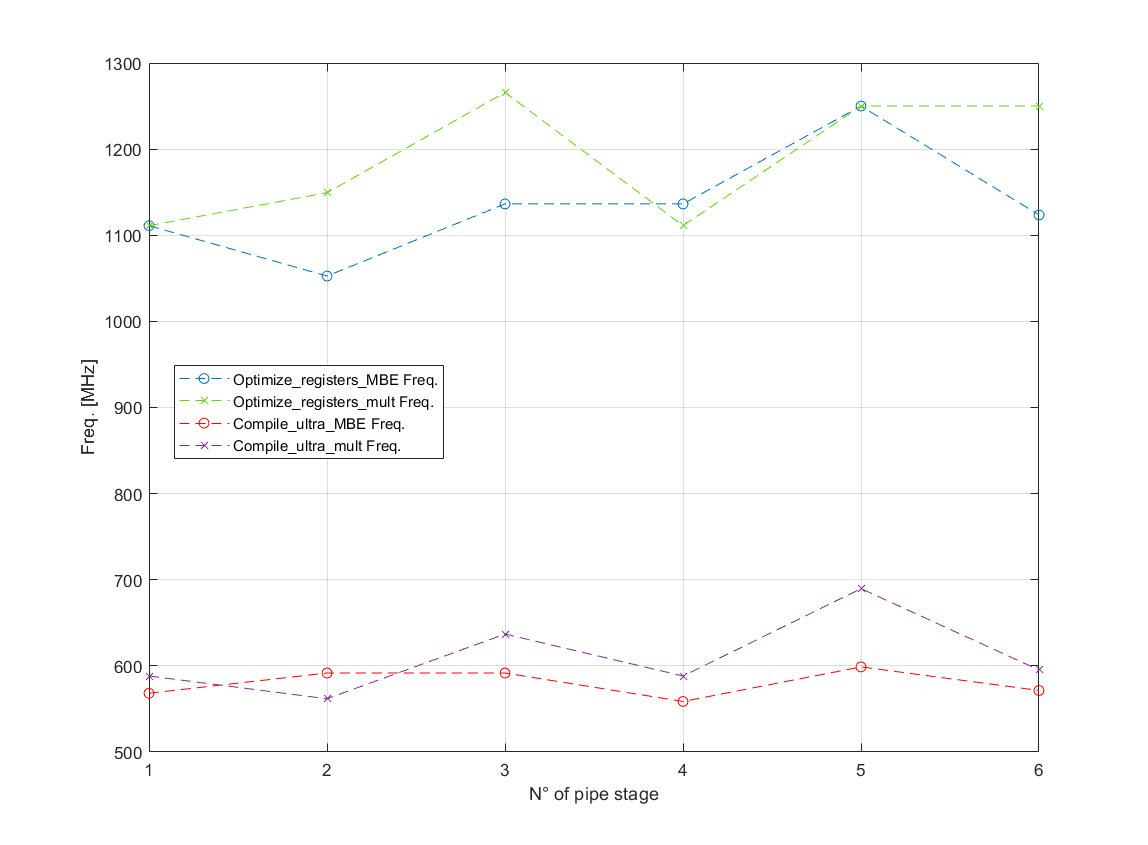
\includegraphics[scale=0.4]{mult_vs_MBE.png}
	\caption{Fre. comparison: base\_version vs MBE\_version}
	\label{fig:MBE vs mult}
\end{figure}
\noindent
For what concerns the area, in Table \ref{tab:area_MBE} 
%are reported all the possible area values for the two different optimizations 
all the possible area values for the two different optimizations are reported, therefore, even all the percentage increases with respect to the "base version" case with one stage of registers at the output of the generic multiplier are present.
\newline As one can see from the data, in both cases the area increases with the number of additional pipelining stages and this is obvious because an higher number of registers involves an higher occupied area.\\
Moreover, all the areas with optimize\_register optimization are higher in all cases and the percentage increase is roughly more than double.
\newline
Thus, this suggests that if the aim is to focus on the performance the best option is to adopt the optimize\_register optimization at the expense of an increase of the area, while, if the purpose is to save area at the expense of a lower operating frequency, the compile\_ultra optimization should be chosen .

\newpage
\section{Tables}
\begin{longtable}{*7c}
\caption{Outputs for each simulation}
\label{tab:output simulations}\\
\toprule
 \thead{Base\\version} & \thead{1 added\\register} & \thead{2 added\\registers} & \thead{3 added\\registers} & \thead{4 added\\registers} & \thead{5 added\\registers}  & \thead{6 added\\registers}\\
\midrule
\endfirsthead
 \thead{Base\\version} & \thead{1 added\\register} & \thead{2 added\\registers} & \thead{3 added\\registers} & \thead{4 added\\registers} & \thead{5 added\\registers}  & \thead{6 added\\registers}\\
\midrule
\endhead
\midrule
\endfoot
\bottomrule
\endlastfoot
xxxxxxxx & xxxxxxxx & xxxxxxxx & xxxxxxxx & xxxxxxxx & xxxxxxxx & xxxxxxxx\\
xxxxxxxx & xxxxxxxx & xxxxxxxx & xxxxxxxx & xxxxxxxx & xxxxxxxx & xxxxxxxx\\
xxxxxxxx & xxxxxxxx & xxxxxxxx & xxxxxxxx & xxxxxxxx & xxxxxxxx & xxxxxxxx\\
xxxxxxxx & xxxxxxxx & xxxxxxxx & xxxxxxxx & xxxxxxxx & xxxxxxxx & xxxxxxxx\\
xxxxxxxx & xxxxxxxx & xxxxxxxx & xxxxxxxx & xxxxxxxx & xxxxxxxx & xxxxxxxx\\
00000000 & xxxxxxxx & xxxxxxxx & xxxxxxxx & xxxxxxxx & xxxxxxxx & xxxxxxxx\\
3DC3910D & 00000000 & xxxxxxxx & xxxxxxxx & xxxxxxxx & xxxxxxxx & xxxxxxxx\\
0BC80005 & 3DC3910D & 00000000 & xxxxxxxx & xxxxxxxx & xxxxxxxx & xxxxxxxx\\
3F278DDF & 0BC80005 & 3DC3910D & 00000000 & xxxxxxxx & xxxxxxxx & xxxxxxxx\\
0B100005 & 3F278DDF & 0BC80005 & 3DC3910D & 00000000 & xxxxxxxx & xxxxxxxx\\
3F800000 & 0B100005 & 3F278DDF & 0BC80005 & 3DC3910D & 00000000 & xxxxxxxx\\
0C440004 & 3F800000 & 0B100005 & 3F278DDF & 0BC80005 & 3DC3910D & 00000000\\
3F278DDF & 0C440004 & 3F800000 & 0B100005 & 3F278DDF & 0BC80005 & 3DC3910D\\
0DA20000 & 3F278DDF & 0C440004 & 3F800000 & 0B100005 & 3F278DDF & 0BC80005\\
3DC3910D & 0DA20000 & 3F278DDF & 0C440004 & 3F800000 & 0B100005 & 3F278DDF\\
 & 3DC3910D & 0DA20000 & 3F278DDF & 0C440004 & 3F800000 & 0B100005\\
 &  & 3DC3910D & 0DA20000 & 3F278DDF & 0C440004 & 3F800000\\
 &  &  & 3DC3910D & 0DA20000 & 3F278DDF & 0C440004\\
 &  &  &  & 3DC3910D & 0DA20000 & 3F278DDF\\
 &  &  &  &  & 3DC3910D & 0DA20000\\
 &  &  &  &  &  & 3DC3910D\\
\end{longtable}

\begin{longtable}{*4c}
\caption{Synthesys results for base, CSA and PPARCH versions}
\label{tab:synthesys mult}\\
\toprule
 Parameters&\thead{Base\\version} & \thead{CSA\\version} & \thead{PPARCH\\version}\\
\midrule
\endfirsthead
Parameters& \thead{Base\\version} & \thead{CSA\\version} & \thead{PPARCH\\version}\\
\midrule
\endhead
\midrule
\endfoot
\bottomrule
\endlastfoot
Maximum frequency [MHz] & 632,9 & 232,6 & 606,1 \\
Total cell area [$\mu m^2$] &  4057,8 & 4861,4 & 4009,4 \\
\end{longtable}


\begin{longtable}{*5c}
\caption{Base\_version: Optimize\_registers freq. vs Compile\_ultra freq.}
\label{tab:freq_pipe_opt}\\
\toprule                                         
 \thead{N°\;pipe} & \thead{$T_{ck}$ optimize\_reg \\$[ns]$} & \thead{Freq. optimize\_reg \\ $[MHz]$}  & \thead{$T_{ck}$ compile\_ultra\\ $[ns]$} & \thead{Freq. compile\_ultra \\ $[MHz]$}\\
\midrule
\endfirsthead

 \thead{N°\;pipe} & \thead{$T_{ck}$ \\optimize\_reg \\$[ns]$} & \thead{Freq. optimize\_reg \\ $[MHz]$}  & \thead{$T_{ck}$ compile\_ultra\\ $[ns]$} & \thead{Freq. compile\_ultra \\ $[MHz]$}\\ 
  
\midrule
\endhead
\midrule
\endfoot
\bottomrule
\endlastfoot

0&	1,58&	632,91&	1,58&	632,91 \\ 
1&	0,9	&   1111,11	&1,7&	588,24  \\
2&	0,87&	1149,43	&1,78&	561,80  \\
3&	0,79&	1265,82	&1,57&	636,94  \\
4&	0,9&	1111,11	&1,7&	588,24  \\
5&	0,8&	1250,00	&1,45&	689,66\\
6&	0,8&	1250,00	&1,68&	595,24\\

\end{longtable}




\begin{longtable}{*5c}
\caption{Base\_version: Area report for different pipelining stages and optimizations}
\label{tab:area_mult}\\
\toprule
 \thead{N° pipe}&  \thead{Area optimize\_reg \\$[\mu m^2]$}& \thead{\% Inc.} & \thead{Area compile\_ultra \\$[\mu m^2]$} &  \thead{\% Inc.}\\
 \midrule
\endfirsthead
 \thead{N° pipe}&  \thead{Area optimize\_reg \\$[\mu m^2]$}& \thead{\% Inc.} & \thead{Area compile\_ultra \\$[\mu m^2]$}&  \thead{\% Inc.}\\
\midrule
\endhead
\midrule
\endfoot
\bottomrule
\endlastfoot
0& 4057,83 (no opt) & 0,00 &  4057,83 (no opt)  & 0,00   \\
1&4586,9        	& 13,04 &  4020,57 &				-0,92	\\
2&4697,56       	& 15,77 &  4200,41  	&				3,51	\\
3&5211,74       	& 28,44 &  4485,56  	&				10,54	\\
4&5010,38       	& 23,47 &  4577,59  	&				12,81	\\
5&5506,2        	& 35,69 &  5022,88	 &				23,78	\\
6&5650,9        	& 39,26 &  4935,36	 &				21,63	\\
\end{longtable}	







\begin{longtable}{*5c}
\caption{MBE\_version: Freq. comparison custom and generic BEU\_PP17}
\label{tab:pp_17}\\
\toprule
 \thead{BEU\_PP17}&\thead{$T_{ck}$ optimize\_reg \\$[ns]$} & \thead{Freq. optimize\_reg \\ $[MHz]$}  & \thead{$T_{ck}$ compile\_ultra\\ $[ns]$} & \thead{Freq. compile\_ultra \\ $[MHz]$}\\
\midrule
\endfirsthead
 \thead{BEU\_PP17}&\thead{$T_{ck}$ optimize\_reg \\$[ns]$} & \thead{Freq. optimize\_reg \\ $[MHz]$}  & \thead{$T_{ck}$ compile\_ultra\\ $[ns]$} & \thead{Freq. compile\_ultra \\ $[MHz]$}\\
\midrule
\endhead
\midrule
\endfoot
\bottomrule
\endlastfoot
Custom & 0,92 & 1086,96 & 3,02 & 331,13 \\
Generic &  0,9 & 1111,11 & 1,76 & 568,18 \\
\end{longtable}

\begin{longtable}{*3c}
\caption{MBE\_version: Area comparison custom and generic BEU\_PP17}
\label{tab:area_pp_17}\\
\toprule
 \thead{BEU\_PP17}&  \thead{Area optimize\_reg \\$[\mu m^2]$}&  \thead{Area compile\_ultra \\$[\mu m^2]$}\\
 \midrule
\endfirsthead
 \thead{BEU\_PP17}&  \thead{Area optimize\_reg \\$[\mu m^2]$}&  \thead{Area compile\_ultra \\$[\mu m^2]$}\\
\midrule
\endhead
\midrule
\endfoot
\bottomrule
\endlastfoot
Custom & 7033,57 & 4385,28 \\
Generic & 7033,04 & 5122,36 \\
\end{longtable}



\begin{longtable}{*5c}
\caption{MBE\_version: MBE\_Optimize\_registers freq. vs MBE\_Compile\_ultra freq.}
\label{tab:freq_pipe_opt_MBE}\\
\toprule                                         
 \thead{N°\;pipe} & \thead{$T_{ck}$ optimize\_reg \\$[ns]$} & \thead{Freq. optimize\_reg \\ $[MHz]$}  & \thead{$T_{ck}$ compile\_ultra\\ $[ns]$} & \thead{Freq. compile\_ultra \\ $[MHz]$}\\
\midrule
\endfirsthead

 \thead{N°\;pipe} & \thead{$T_{ck}$ \\optimize\_reg \\$[ns]$} & \thead{Freq. optimize\_reg \\ $[MHz]$}  & \thead{$T_{ck}$ compile\_ultra\\ $[ns]$} & \thead{Freq. compile\_ultra \\ $[MHz]$}\\ 
  
\midrule
\endhead
\midrule
\endfoot
\bottomrule
\endlastfoot

1&	0,9  &  1111,11	&1,76&	568,18  \\
2&	0,95 &	1052,63	&1,69&	591,72  \\
3&	0,88 &	1136,36	&1,69&	591,72  \\
4&	0,88 &	1136,36	&1,79&	558,66  \\
5&	0,8  &	1250,00	&1,67&	598,80\\
6&	0,89  &	1123,60	&1,75&	571,43\\


\end{longtable}



\begin{longtable}{*5c}
\caption{MBE\_version: Area report for different pipelining stages and optimizations}
\label{tab:area_MBE}\\
\toprule
  \thead{N° pipe}&  \thead{Area optimize\_reg \\$[\mu m^2]$}& \thead{\% Inc.} & \thead{Area compile\_ultra \\$[\mu m^2]$} &  \thead{\% Inc.}\\
 \midrule
\endfirsthead
 \thead{N° pipe}&  \thead{Area optimize\_reg \\$[\mu m^2]$}&  \thead{\% Inc.} & \thead{Area compile\_ultra \\$[\mu m^2]$} &  \thead{ \% Inc.}\\
\midrule
\endhead
\midrule
\endfoot
\bottomrule
\endlastfoot
1 & 7033,04 & 73,32	&	5122,36 & 26,23\\
2 & 7196,63 & 77,35	&	5337,82 & 31,54\\
3 & 7530,46 & 85,58	&	5516,31 & 35,94\\
4 & 7675,16 & 89,14	&	5580,68 & 37,53\\
5 & 7991,17 & 96,93	&	5886,85 & 45,07\\
6 & 7857,91 & 93,65	&	6044,05 & 48,95\\
\end{longtable}		






\end{document}
  
